
% LaTeX Beamer file automatically generated from DocOnce
% https://github.com/hplgit/doconce

%-------------------- begin beamer-specific preamble ----------------------

\documentclass{beamer}

\usetheme{red_plain}
\usecolortheme{default}

% turn off the almost invisible, yet disturbing, navigation symbols:
\setbeamertemplate{navigation symbols}{}

% Examples on customization:
%\usecolortheme[named=RawSienna]{structure}
%\usetheme[height=7mm]{Rochester}
%\setbeamerfont{frametitle}{family=\rmfamily,shape=\itshape}
%\setbeamertemplate{items}[ball]
%\setbeamertemplate{blocks}[rounded][shadow=true]
%\useoutertheme{infolines}
%
%\usefonttheme{}
%\useinntertheme{}
%
%\setbeameroption{show notes}
%\setbeameroption{show notes on second screen=right}

% fine for B/W printing:
%\usecolortheme{seahorse}

\usepackage{pgf,pgfarrows,pgfnodes,pgfautomata,pgfheaps,pgfshade}
\usepackage{graphicx}
\usepackage{epsfig}
\usepackage{relsize}

\usepackage{fancybox}  % make sure fancybox is loaded before fancyvrb

\usepackage{fancyvrb}
%\usepackage{minted} % requires pygments and latex -shell-escape filename
%\usepackage{anslistings}
%\usepackage{listingsutf8}

\usepackage{amsmath,amssymb,bm}
%\usepackage[latin1]{inputenc}
\usepackage[T1]{fontenc}
\usepackage[utf8]{inputenc}
\usepackage{colortbl}
\usepackage[english]{babel}
\usepackage{tikz}
\usepackage{framed}
% Use some nice templates
\beamertemplatetransparentcovereddynamic

% --- begin table of contents based on sections ---
% Delete this, if you do not want the table of contents to pop up at
% the beginning of each section:
% (Only section headings can enter the table of contents in Beamer
% slides generated from DocOnce source, while subsections are used
% for the title in ordinary slides.)
\AtBeginSection[]
{
  \begin{frame}<beamer>[plain]
  \frametitle{}
  %\frametitle{Outline}
  \tableofcontents[currentsection]
  \end{frame}
}
% --- end table of contents based on sections ---

% If you wish to uncover everything in a step-wise fashion, uncomment
% the following command:

%\beamerdefaultoverlayspecification{<+->}

\newcommand{\shortinlinecomment}[3]{\note{\textbf{#1}: #2}}
\newcommand{\longinlinecomment}[3]{\shortinlinecomment{#1}{#2}{#3}}

\definecolor{linkcolor}{rgb}{0,0,0.4}
\hypersetup{
    colorlinks=true,
    linkcolor=linkcolor,
    urlcolor=linkcolor,
    pdfmenubar=true,
    pdftoolbar=true,
    bookmarksdepth=3
    }
\setlength{\parskip}{0pt}  % {1em}

\newenvironment{doconceexercise}{}{}
\newcounter{doconceexercisecounter}
\newenvironment{doconce:movie}{}{}
\newcounter{doconce:movie:counter}

\newcommand{\subex}[1]{\noindent\textbf{#1}}  % for subexercises: a), b), etc

%-------------------- end beamer-specific preamble ----------------------

% Add user's preamble




% insert custom LaTeX commands...

\raggedbottom
\makeindex

%-------------------- end preamble ----------------------

\begin{document}

% endif for #ifdef PREAMBLE



% ------------------- main content ----------------------



% ----------------- title -------------------------

\title{Education for the future}

% ----------------- author(s) -------------------------

\author{Morten Hjorth-Jensen\inst{1,2}
\and
Anders Malthe-Sørenssen\inst{1}}
\institute{Department of Physics, University of Oslo\inst{1}
\and
Department of Physics and Astronomy, Michigan State University, USA\inst{2}}
% ----------------- end author(s) -------------------------

\date{September 2 2015,
% <optional titlepage figure>
}

\begin{frame}[plain,fragile]
\titlepage
\end{frame}

\begin{frame}[plain,fragile]
\frametitle{Present and future education}

\begin{block}{}

\begin{itemize}
\item \textbf{Research-based education}, from undergraduate studies to a PhD: \href{{http://www.mn.uio.no/fysikk/english/research/groups/computational/index.html}}{The Computational Physics group at the University of Oslo} as example

\item Future challenges and directions
\end{itemize}

\noindent
\end{block}
\begin{block}{Takeaway message }
Excellent research depends on excellent education --- and vice versa!
% A successful research program cannot be disconnected from education and vice versa
\end{block}
\end{frame}

\begin{frame}[plain,fragile]
\frametitle{The role of computations, from education to society}

\begin{block}{}
\textbf{Computations are central to our 
basic understanding of nature and to technological advances}.
UiO's strength in computational science (education and research)
has the potential to make UiO a top European university.
\end{block}

\begin{block}{Examples }
\begin{itemize}
\item \textbf{Nanotech and Materials}: quantum physical systems in nanotechnology; characteristics of new materials; semi-conductor devices and quantum computers

\item \textbf{The smallest particles in nature}: subatomic physics at its smallest length scale

\item \textbf{And the largest}: simulating galaxies and the evolution of the universe

\item \textbf{Life science}: cancer treatment and how the brain works

\item \textbf{Geosciences}: predicting climate changes and this week's weather, simulating natural disasters

\item \textbf{Finance}: assessing risk in the insurance and financial industry

\item and many many more
\end{itemize}

\noindent
\end{block}
\end{frame}

\begin{frame}[plain,fragile]
\frametitle{Modeling and computations as a way to enhance algorithminc thinking}

\begin{block}{}
\textbf{Algorithm} :
A set of instructions to solve a problem.
\end{block}

\begin{block}{}
\textbf{Algorithmic thinking applies to all disciplines. It}
\begin{itemize}
\item Enhances instruction-based teaching

\item Introduces research-based teaching  from day one

\item Triggers further insights in scientific problems

\item Emphasizes validation and verification of scientific results, and integrates science ethics in a natural way

\item Ensures good working practices from day one!
\end{itemize}

\noindent
\end{block}
\end{frame}

\begin{frame}[plain,fragile]
\frametitle{What does computing mean?}

\begin{block}{}

\textbf{Computing means solving scientific problems using computers. It covers numerical as well as symbolic computing. Computing is also about developing an understanding of the scientific process by enhancing the algorithmic thinking when solving problems.}
\end{block}

\begin{block}{Computing competence is about: }

\begin{itemize}
\item derivation, verification, and implementation of algorithms

\item understanding what can go wrong with algorithms

\item overview of important, known algorithms

\item understanding how algorithms are used to solve complicated problems

\item reproducible science and ethics

\item algorithmic thinking for gaining deeper insights about scientific problems
\end{itemize}

\noindent
All these elements (and many more) aid students in maturing and gaining a better understanding of the scientific process \emph{per se}.
\end{block}
\end{frame}

\begin{frame}[plain,fragile]
\frametitle{Computing and research-based education}

\begin{block}{}
A computational approach allows us to introduce research concepts and engage students in research from \emph{day one}.
\end{block}


\begin{block}{What should the education contain? }

\begin{itemize}
\item Theory + experiment + simulation is the norm in research and industry

\item Modeling of real, complex systems with no simple answers

\item Insight and understanding of fundamental principles and laws

\item Visualization, presentation, discussion, interpretation, and critical analysis of results

\item Development of a sound ethical attitude to own and other's work

\item Enhanced reasoning about the scientific method

\item Individually tailored education in order to let students  realize their full potentials and discover their creative powers
\end{itemize}

\noindent
This is what we do in the \href{{http://www.mn.uio.no/fysikk/english/research/groups/computational/index.html}}{Computational Physics group at UiO}!
\end{block}
\end{frame}

\begin{frame}[plain,fragile]
\frametitle{\href{{http://www.mn.uio.no/fysikk/english/research/groups/computational/index.html}}{Computational Physics group at UiO}; our visions}

\begin{columns}
\column{0.4\textwidth}
\begin{block}{}
Physics students can \textbf{pose and solve problems} that combine \textbf{physical insights} with \textbf{mathematical tools} and now also \textbf{computational skills}.
Essential for multi-disciplinary programs.
% This provides a unique combination of applied and theoretical knowledge and skills. These features are invaluable for the development of multi-disciplinary educational and research programs.
\end{block}

\column{0.6\textwidth}
% inline figure
\centerline{
\includegraphics[width=1.0\linewidth]{fig-future/computer_nerd2.jpg}}



\end{columns}
\end{frame}

\begin{frame}[plain,fragile]
\frametitle{A social and scientific learning environment}

\begin{block}{}
\textbf{Goal: Students should realize their full potentials and discover their creative powers}

\begin{itemize}
 \item Students come with different dreams, ambitions, aspirations and topics they wish to study, our approach is to tailor the education to all these aspects

 \item Our motto: foster students who are better than their supervisors

 \item Emphasis is on learning and getting new insights

 \item Students and teachers help each other

 \item Students with different backgrounds and needs can thrive socially and scientifically

 \item Non-competitive and generous environment
% Not a competitive environment, but a drive and enthusiam for sharing and developing knowledge. This is an important element for the  success of for example multi-disciplinary projects
\end{itemize}

\noindent
\end{block}
\end{frame}

\begin{frame}[plain,fragile]
\frametitle{We develop a social and scientific learning environment}

\begin{block}{}
\begin{itemize}
\item We target bachelor, MSc and PhD students

\item Project-oriented work where students develop and mature their own ideas, with an individually tailored approach to each student

\item Office space with desktops to every student and large common room for recreational activities (meals, gaming, movies)

\item Many students collaborate on similar  thesis topics and \href{{http://www.dn.no/talent/2014/06/12/Utdannelse/sommervikar-ble-toppforsker}}{publish in top scientific journals}
\end{itemize}

\noindent
\end{block}
\end{frame}

\begin{frame}[plain,fragile]
\frametitle{Features of the Computational Physics group}

\begin{block}{}
\begin{itemize}
\item Our students have made significant contributions to  the \href{{http://www.mn.uio.no/english/about/collaboration/cse/}}{Computing in Science Education}  (UiO education prize in 2011) by developing exercises and participating in educational projects at the MN faculty

\item Our students have also developed educational \href{{http://www.mn.uio.no/fysikk/om/aktuelt/aktuelle-saker/2015/realfagsapper.html}}{tools and applications for understanding complicated physical problems}

\item A group of PhD students is now developing \href{{https://github.com/CINPLA/ibvcse}}{new textbooks for Computational Life Science}

\item 2005-2015: $> 60$ students have finalized their master's theses and 60\% have continued with PhD studies

\item Many students don't want to leave the group after finishing their studies
\end{itemize}

\noindent
\end{block}
\end{frame}

\begin{frame}[plain,fragile]
\frametitle{Investing in equipment for research and education}

\begin{columns}
\column{0.2\textwidth}
\begin{block}{}
Large screens for visualizing and presenting scientific results. And gaming and other social activities. 
\begin{itemize}
\item Here we see two students displaying results from large-scale simulations of molecules in materials

\item With 3D visualization tools one can see structures which where not possible until recently
\end{itemize}

\noindent
\end{block}

\column{0.8\textwidth}
% inline figure
\centerline{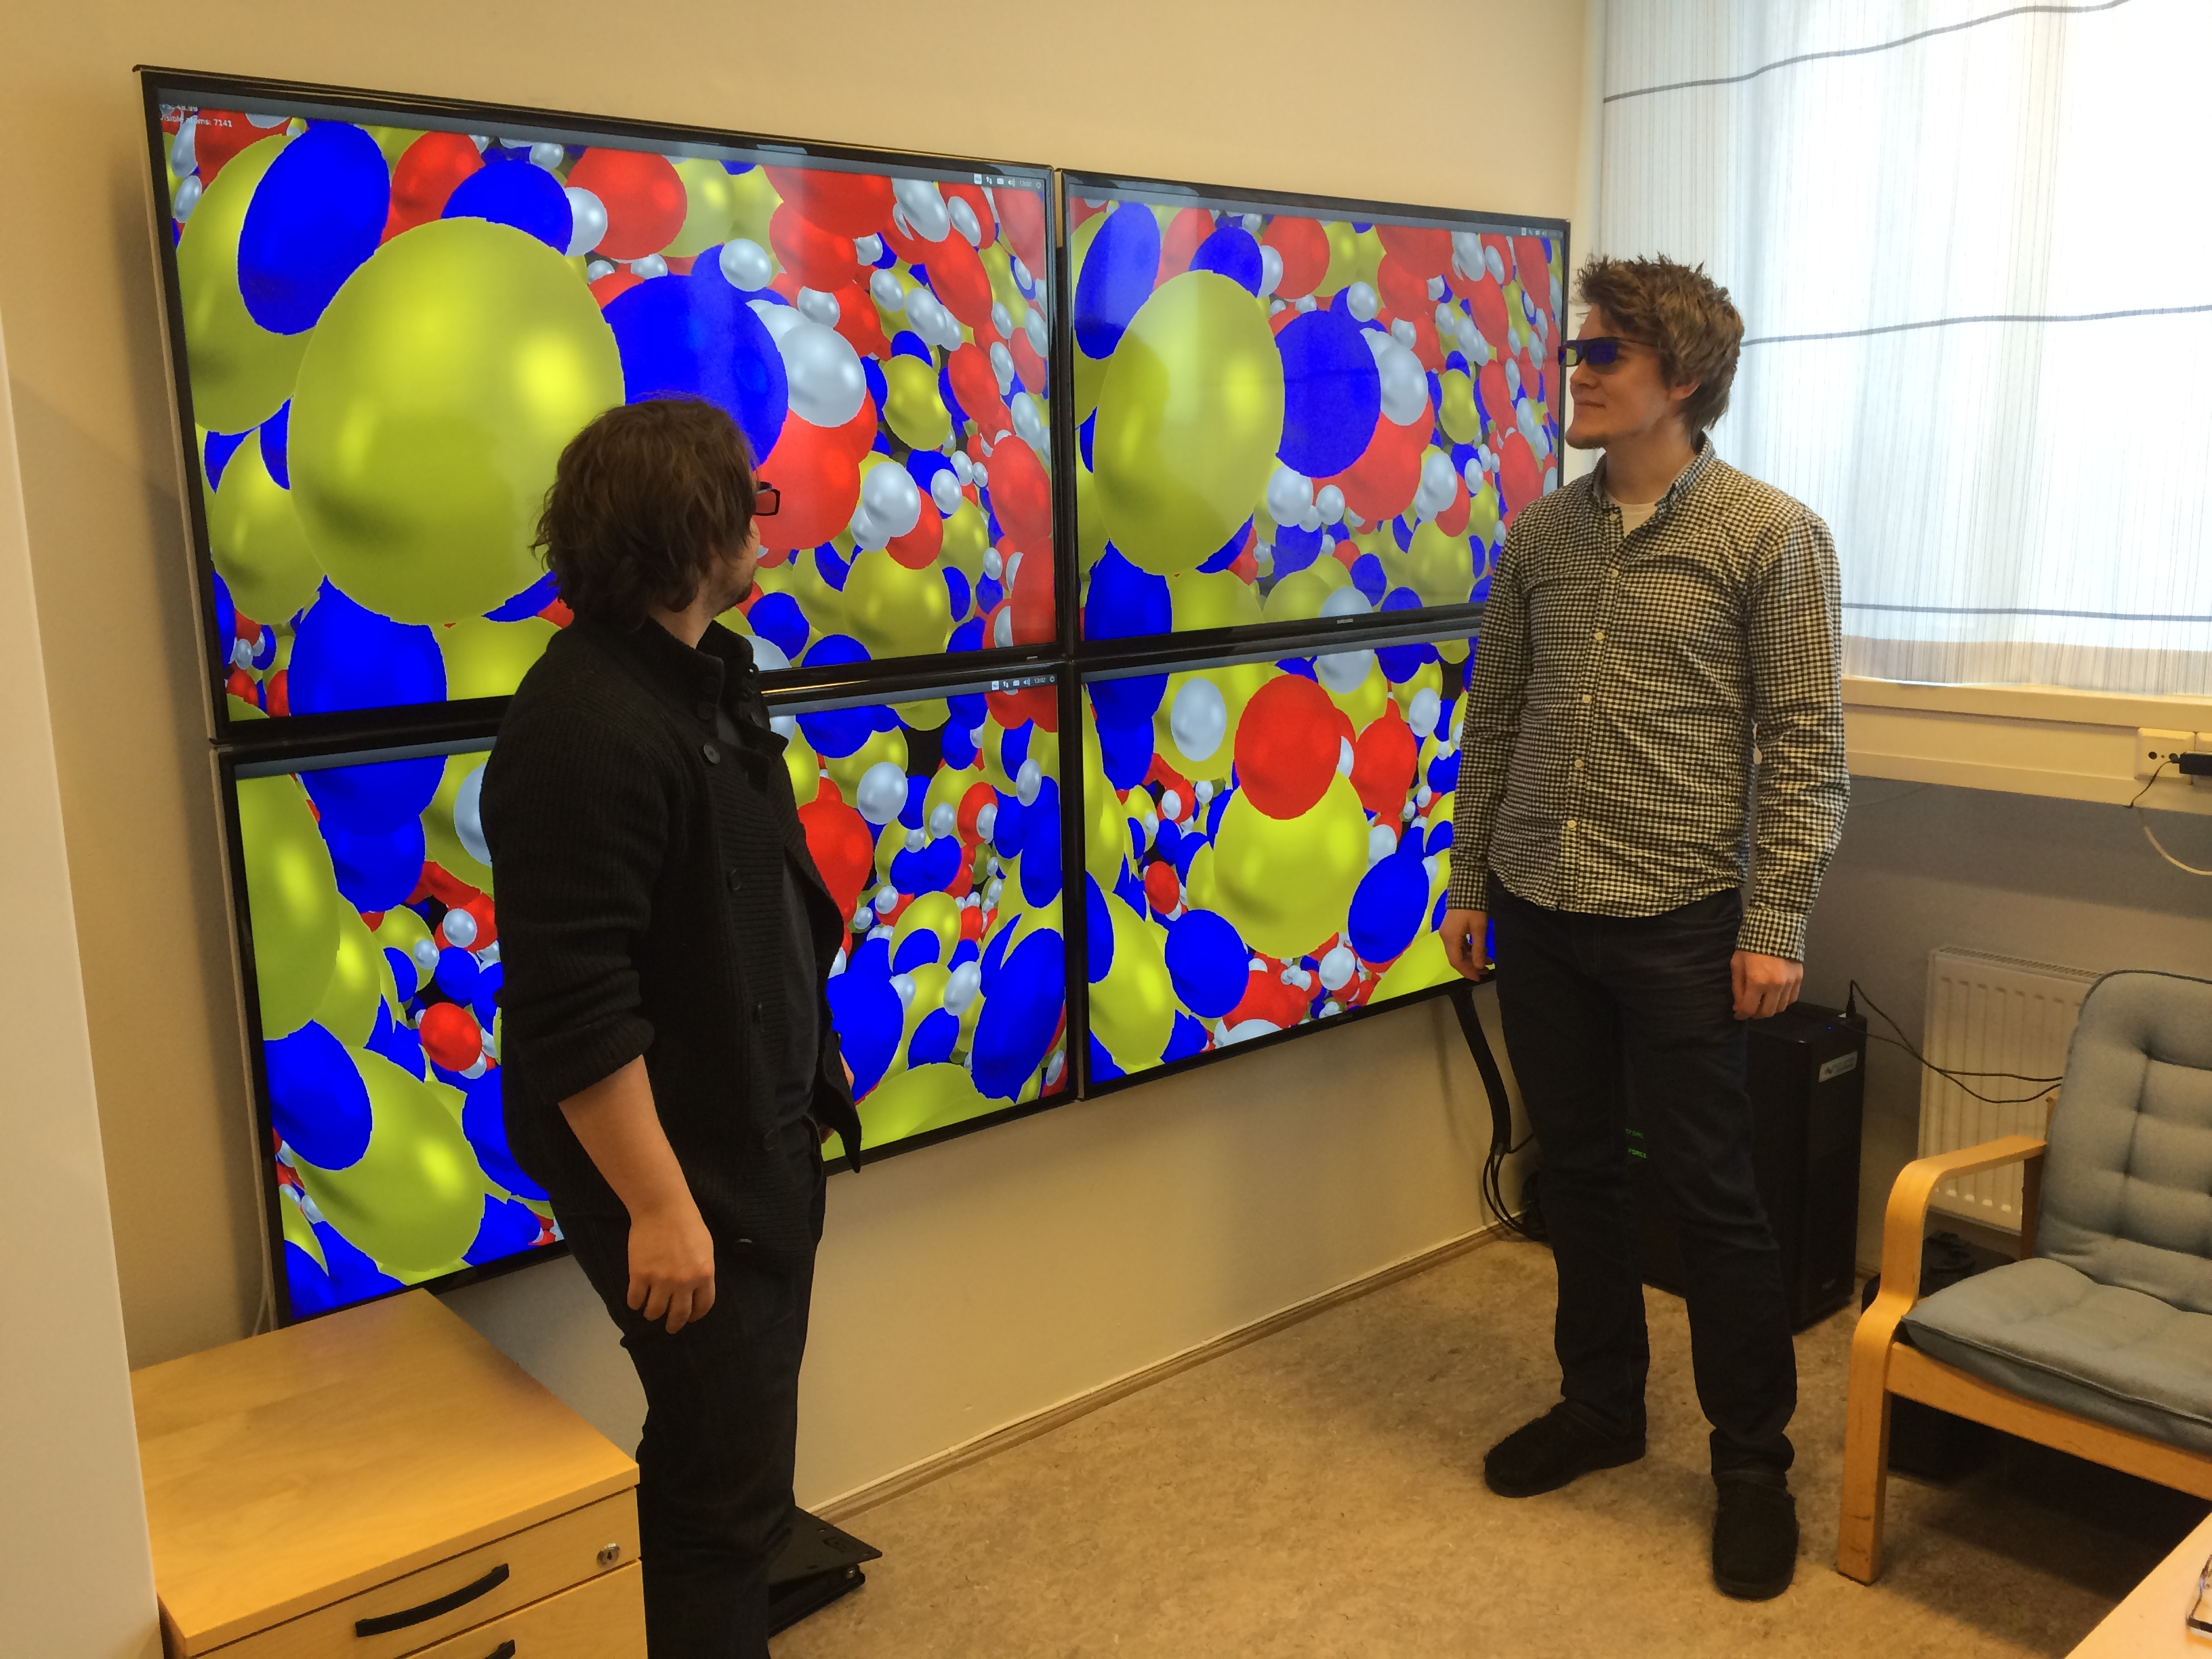
\includegraphics[width=1.0\linewidth]{fig-future/visualize.jpg}}



\end{columns}
\end{frame}

\begin{frame}[plain,fragile]
\frametitle{Building a local supercomputing cluster from titan.uio.no}

\begin{columns}
\column{0.2\textwidth}
\begin{block}{Our supercomuting cluster }
When UiO's previous supercomputing cluster (titan.uio.no) was replaced by \textbf{abel.uio.no}, we got 200 nodes for free from USIT and built our own supercomputer. The value in 2006 of all the equipment was close to eight MNOK.
\begin{itemize}
\item It helps students run and develop programs for large-scale problems locally

\item A successful program can then run on larger national and international supercomputers

\item Students run and maintain the local supercomputer

\item Used in regular courses as well
\end{itemize}

\noindent
\end{block}

\column{0.8\textwidth}
% inline figure
\centerline{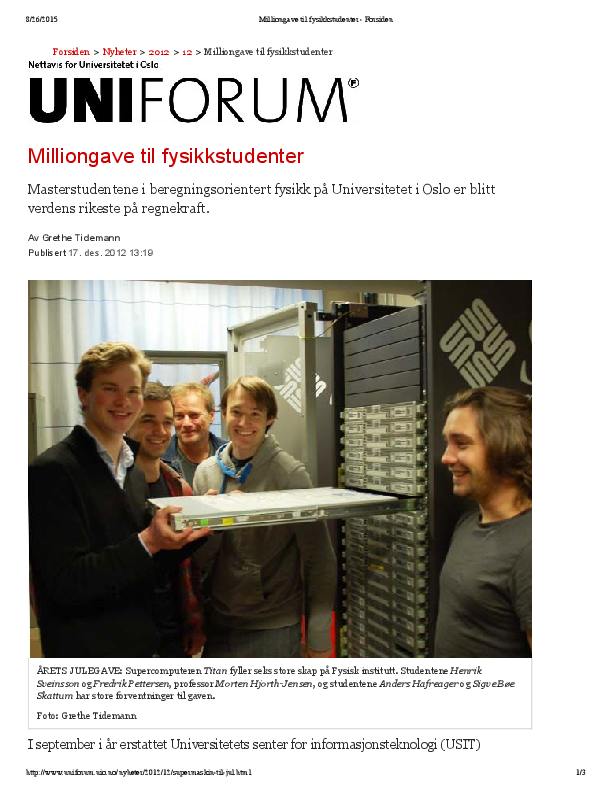
\includegraphics[width=1.0\linewidth]{fig-future/uniforum-0.png}}



\end{columns}
\end{frame}

\begin{frame}[plain,fragile]
\frametitle{Undergraduate student publishes in PNAS}

\begin{columns}
\column{0.1\textwidth}
\begin{block}{Participating in research from day one! }
\begin{itemize}
\item Bachelor and master students publish in scientific journals 

\item Undergraduate students are exposed to research at early stages, often working with more advanced students

\item Students are exposed to all stages of the scientific process

\item Projects are tailored to the interests of the students

\item Focus on insights and sharing knowledge
\end{itemize}

\noindent
\end{block}

\column{0.9\textwidth}
% inline figure
\centerline{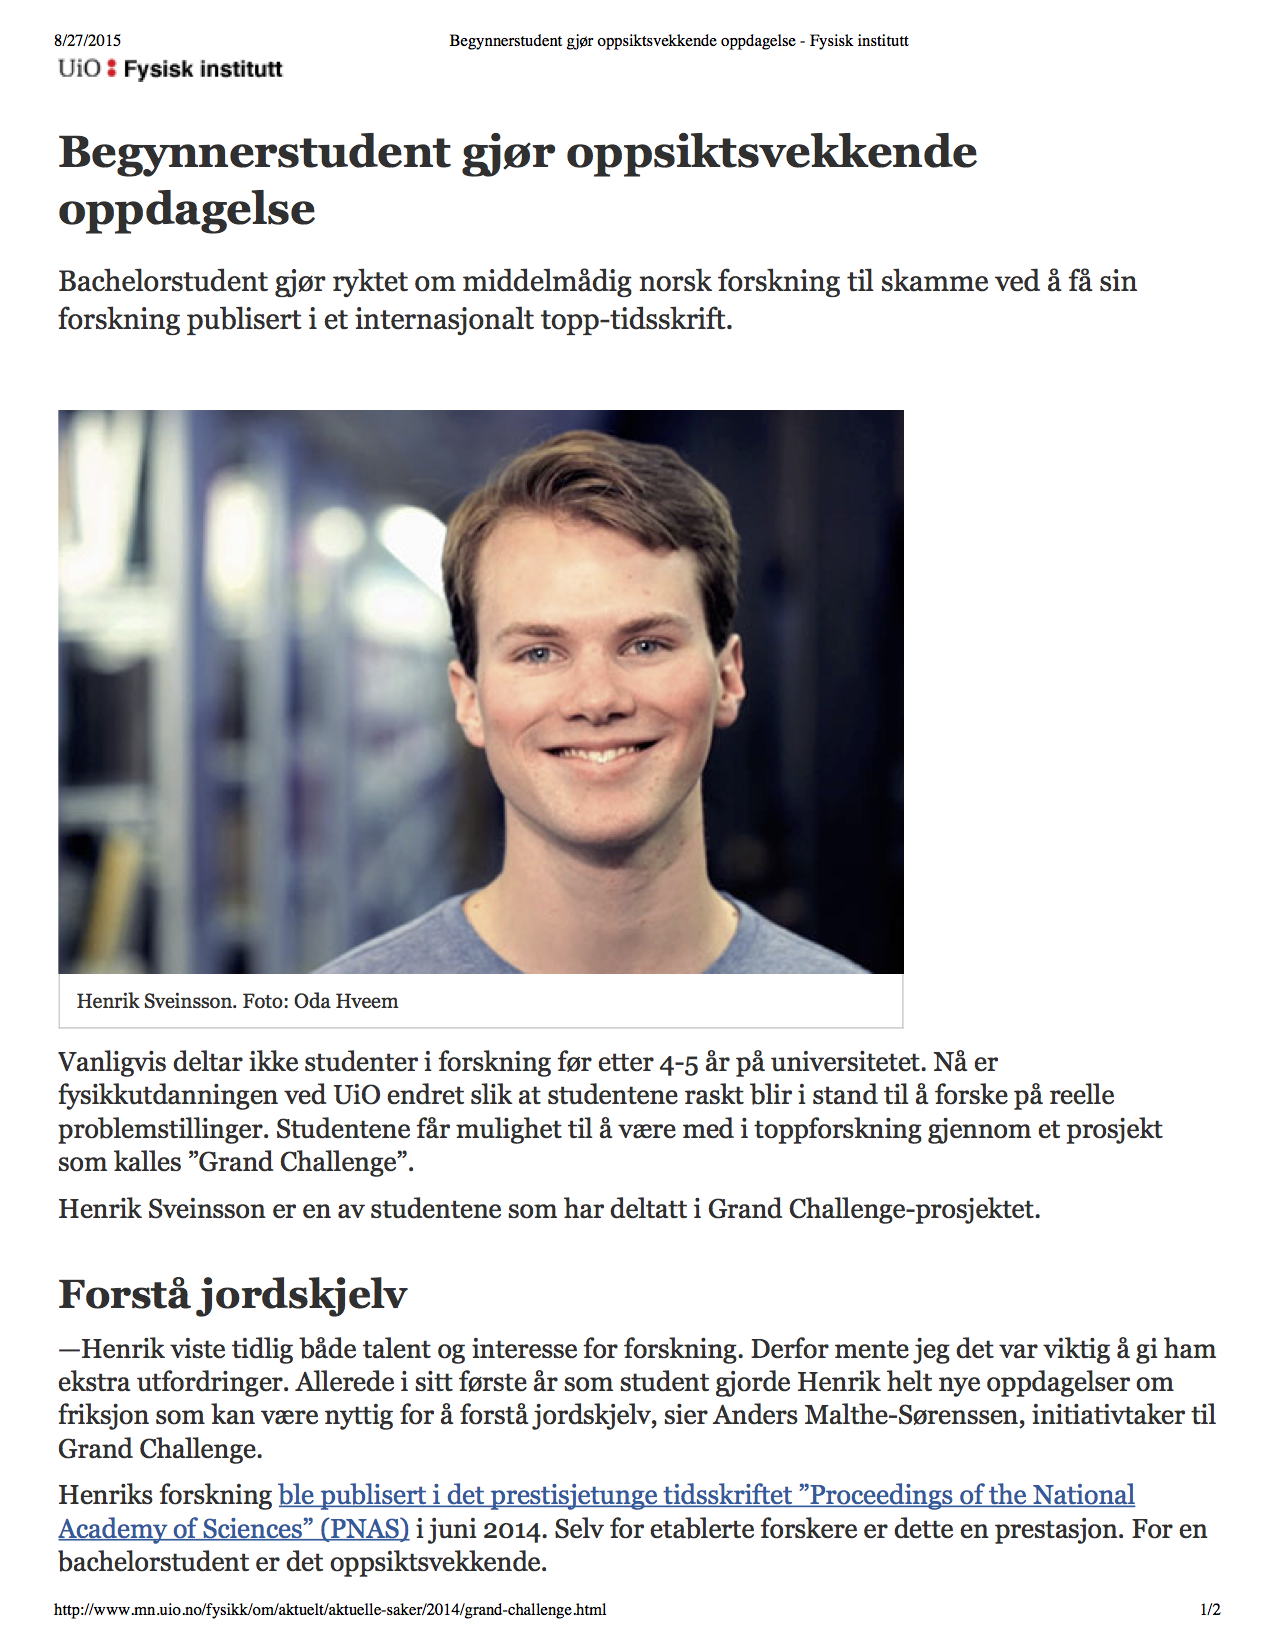
\includegraphics[width=1.0\linewidth]{fig-future/pnas.png}}



\end{columns}
\end{frame}

\begin{frame}[plain,fragile]
\frametitle{The computational revolution in science in society}

\begin{block}{}
\begin{itemize}
\item Computing will affect all aspects of society - and should also play a key role in research and education in our society

\item Possible large shifts with the advent of automation
\end{itemize}

\noindent
\end{block}

\begin{block}{}
\begin{itemize}
\item Present and future problems involve complex systems

\item Require a multi-disciplinary approach

\item Collaboration and team work using computational tools
\end{itemize}

\noindent
\end{block}

\begin{block}{}
\begin{itemize}
\item To stay competitive as a society we need computing competence integrated in all fields – for both research and education!

\item We need candidates with the right multi-disciplinary background and skills in computational thinking
\end{itemize}

\noindent
\end{block}
\end{frame}

\begin{frame}[plain,fragile]
\frametitle{Multiscale modeling is the big open research question in the 21st century}

\begin{block}{}
\begin{itemize}
\item Present and future problems, unlike traditional science and engineering, involve complex systems with many distinct physical processes

\item The wide open research topic of this century, both in industry and at universities, is how to effectively couple processes across different length and energy scales

\item Progress will rely on a \emph{multi-disciplinary} approach
\end{itemize}

\noindent
\end{block}

\begin{block}{}
We need to foster candidates with the right
multi-disciplinary background and computational thinking!
\end{block}
\end{frame}

\begin{frame}[plain,fragile]
\frametitle{UiO has a unique opportunity to become a Leading European University}

\begin{block}{}
UiO's strength in computational science (education and research)
has the potential to make UiO a top European university

\begin{itemize}
\item We must educate the competence needed

\item We are in a unique position to do so --- across all fields!
\end{itemize}

\noindent
\end{block}

\begin{block}{How to achieve this }
\begin{itemize}
\item Establish  a new center/department with focus on computational science and its applications to a wide range of fields (natural science, medicine, social sciences, humanities, applied research etc)

\item Hire ten young professors (age $< 40$) dedicated to innovative \emph{computational} research and education

\item Establish another ten professorships with  shared positions between the  new department and the discipline-specific department

\item Establish  best practices for computational and educational innovations, with a particular focus on  new learning material and real incentives
\end{itemize}

\noindent
\end{block}

\textbf{The process must start now} in order not to lose momentum.
\end{frame}

\begin{frame}[plain,fragile]
\frametitle{Our takeaway messages}

\begin{block}{}
\begin{itemize}
\item Computing plays and will play an even more important role in society --– and this must be reflected in research and education

\item Our program builds in this and allows students to realize their potential and unleash their creativity

\item Social and scientific activities in harmony

\item UiO is in a unique position to develop a leading research and educational activity --- if we act now
\end{itemize}

\noindent
\end{block}
\end{frame}

\begin{frame}[plain,fragile]
\frametitle{Computational Physics and  the Computing in Science Education project (UiO educational prize in 2011)}

\begin{block}{}
The results, insights, ideas and thoughts presented here, would have been impossible without the infinitely many  interactions with colleagues in the \href{{http://www.mn.uio.no/english/about/collaboration/cse/}}{Computing in Science Education} project \textbf{and all our fantastisc students who continuously give us new insights! Thanks}
\end{block}
\begin{columns}
\column{0.4\textwidth}
\begin{block}{}
\begin{itemize}
\item Hans Petter Langtangen

\item Knut Mørken

\item Arnt Inge Vistnes

\item Oyvind Ryan

\item Solveig Kristensen and Annik Myhre

\item Hanne Sølna
\end{itemize}

\noindent
\end{block}

\column{0.6\textwidth}
% inline figure
\centerline{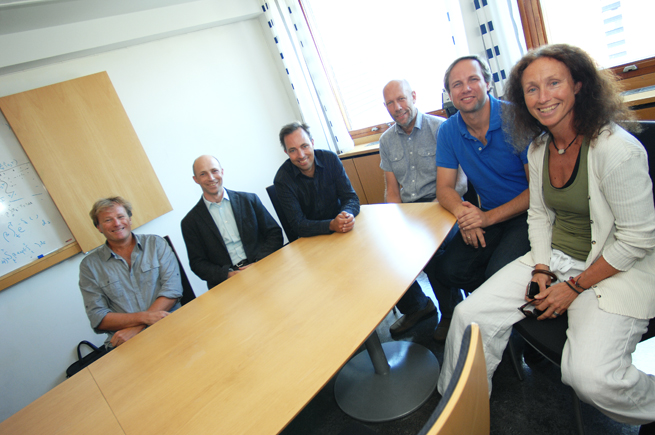
\includegraphics[width=1.0\linewidth]{fig-future/thegang.jpg}}



\end{columns}
\end{frame}

\end{document}
